    \documentclass[dvipsnames]{beamer}
    \usetheme{Madrid}
    \usefonttheme{professionalfonts}
    \usepackage{
        amsmath,
        amssymb,
        fouriernc, % fourier font w/ new century book
        fancyhdr, % page styling
        lastpage, % footer fanciness
        hyperref, % various links
        setspace, % line spacing
        amsthm, % newtheorem and proof environment
        mathtools, % \Aboxed for boxing inside aligns, among others
        float, % Allow [H] figure env alignment
        enumerate, % Allow custom enumerate numbering
        graphicx, % allow includegraphics with more filetypes
        wasysym, % \smiley!
        upgreek, % \upmu for \mum macro
        listings, % writing TrueType fonts and including code prettily
        tikz, % drawing things
        booktabs, % \bottomrule instead of hline apparently
        cancel % can cancel things out!
    }
    \usepackage[
        labelfont=bf, % caption names are labeled in bold
        font=scriptsize % smaller font for captions
    ]{caption}
    \usepackage[font=scriptsize]{subcaption} % subfigures

    \newcommand*{\scinot}[2]{#1\times10^{#2}}
    \newcommand*{\dotp}[2]{\left<#1\,\middle|\,#2\right>}
    \newcommand*{\rd}[2]{\frac{\mathrm{d}#1}{\mathrm{d}#2}}
    \newcommand*{\pd}[2]{\frac{\partial#1}{\partial#2}}
    \newcommand*{\rtd}[2]{\frac{\mathrm{d}^2#1}{\mathrm{d}#2^2}}
    \newcommand*{\ptd}[2]{\frac{\partial^2 #1}{\partial#2^2}}
    \newcommand*{\md}[2]{\frac{\mathrm{D}#1}{\mathrm{D}#2}}
    \newcommand*{\pvec}[1]{\vec{#1}^{\,\prime}}
    \newcommand*{\svec}[1]{\vec{#1}\;\!}
    \newcommand*{\bm}[1]{\boldsymbol{\mathbf{#1}}}
    \newcommand*{\ang}[0]{\;\text{\AA}}
    \newcommand*{\mum}[0]{\;\upmu \mathrm{m}}
    \newcommand*{\at}[1]{\left.#1\right|}

    \let\Re\undefined
    \let\Im\undefined
    \DeclareMathOperator{\Res}{Res}
    \DeclareMathOperator{\Re}{Re}
    \DeclareMathOperator{\Im}{Im}
    \DeclareMathOperator{\Log}{Log}
    \DeclareMathOperator{\Arg}{Arg}
    \DeclareMathOperator{\Tr}{Tr}
    \DeclareMathOperator{\E}{E}
    \DeclareMathOperator{\Var}{Var}
    \DeclareMathOperator*{\argmin}{argmin}
    \DeclareMathOperator*{\argmax}{argmax}
    \DeclareMathOperator{\sgn}{sgn}
    \DeclareMathOperator{\diag}{diag\;}

    \DeclarePairedDelimiter\bra{\langle}{\rvert}
    \DeclarePairedDelimiter\ket{\lvert}{\rangle}
    \DeclarePairedDelimiter\abs{\lvert}{\rvert}
    \DeclarePairedDelimiter\ev{\langle}{\rangle}
    \DeclarePairedDelimiter\p{\lparen}{\rparen}
    \DeclarePairedDelimiter\s{\lbrack}{\rbrack}
    \DeclarePairedDelimiter\z{\lbrace}{\rbrace}

    % \everymath{\displaystyle} % biggify limits of inline sums and integrals
    \tikzstyle{circ} % usage: \node[circ, placement] (label) {text};
        = [draw, circle, fill=white, node distance=3cm, minimum height=2em]
    \definecolor{commentgreen}{rgb}{0,0.6,0}
    \lstset{
        basicstyle=\ttfamily\footnotesize,
        frame=single,
        numbers=left,
        showstringspaces=false,
        keywordstyle=\color{blue},
        stringstyle=\color{purple},
        commentstyle=\color{commentgreen},
        morecomment=[l][\color{magenta}]{\#}
    }

\begin{document}

\begin{frame}
    \frametitle{Review}

    \begin{columns}
        \begin{column}{0.5\textwidth}
            \begin{itemize}
                \item Linear: $\nu = 0$ has $S_{px}(z) = S_{px, 0}$ great
                    prediction. Fit $\vec{u}$ for $\nu \neq 0$ as well, though
                    not $S_{px}(z)$ yet (\textbf{Updated!}).

                \item In nonlinear, review: expect deposited flux $\Delta S_{px}
                    = S_{px, 0}$ incident/generated flux.

                \item Instead, observe $\Delta S_{px} < S_{px, 0}$, and moreover
                    $S_{px}$ far from critical layer changing over time!
            \end{itemize}
        \end{column}
        \begin{column}{0.5\textwidth}
            \begin{itemize}
                \item Last week: defined some
                    \begin{equation}
                        \delta u_z = \frac{u_z - u_{z, 0}
                            - \ev*{u_z}_x}{\abs*{u_{z, 0}}},
                    \end{equation}
                    deviation (new: subtracting mean flow too), computed RMS\@.
                    Found higher RMS for lower $\nu$.

                \item Could it be $\ev*{\dots}_x$ vs $\ev*{\dots}_t$?

                \item Objective: understand ``reflection''?
            \end{itemize}
        \end{column}
    \end{columns}
\end{frame}

\begin{frame}
    \frametitle{Overview}

    \begin{itemize}
        \item Understand exactly how much flux is being absorbed at the critical
            layer:
            \begin{itemize}
                \item Can the decreased flux absorption be explained by
                    viscous dissipation before the critical alyer alone?

                \item Compare predictions of $\pd{z_c}{t}$ to the observed
                    $\Delta S_{px}$ at the critical layer.
            \end{itemize}

        \item Understand nature of ``reflection'', why cannot see in certain
            simulations.
    \end{itemize}
\end{frame}

\begin{frame}
    \frametitle{Results}
    \framesubtitle{Linear}

    Had great $u_z$ fits including viscosity (error $\sim 3-5\%$), but did not
    show great $S_{px}(z; \nu)$ fits last week. Here they are!
    \begin{figure}[t]
        \centering
        \includegraphics[width=0.7\textwidth]{../sims/2d_3_final/snapshots_lin_1/fluxes.png}
        \caption{Fits linear $S_{px}(z; \nu)$.}
    \end{figure}
\end{frame}

\begin{frame}
    \frametitle{Results}
    \framesubtitle{Mean Flow and Flux}

    \begin{columns}
        \begin{column}{0.5\textwidth}
            \begin{figure}[t]
                \centering
                \includegraphics[width=\textwidth]{../sims/2d_3_final/snapshots_nl_4/fluxes.png}
            \end{figure}
        \end{column}
        \begin{column}{0.5\textwidth}
            \begin{itemize}
                \item Last week: Evolution of $\ev*{u_x}_x(t),
                    \ev*{S_{px}}_x(t)$ at different times. Note flux seems to
                    decrease over time throughout domain.

                \item Bottom panel, solid lines are time slices, dotted lines
                    indicate averaging over $\sim \frac{2\pi}{\omega}$ one
                    period (6 times), thick line is linear viscous prediction.

                \item Shaded grey indicates one vertical wavelength.
            \end{itemize}
        \end{column}
    \end{columns}
\end{frame}

\begin{frame}
    \frametitle{Results}
    \framesubtitle{Mean Flow and Flux}

    \begin{columns}
        \begin{column}{0.5\textwidth}
            \begin{figure}[t]
                \centering
                \includegraphics[width=\textwidth]{../sims/2d_3_final/snapshots_nl_1/fluxes.png}
            \end{figure}
        \end{column}
        \begin{column}{0.5\textwidth}
            \begin{itemize}
                \item More damped for comparison ($\nu \to 7\nu/3$).

                \item Note that $S_{px}$ does not change much over time, general
                    trend matches viscous linear decrease.
            \end{itemize}
        \end{column}
    \end{columns}
\end{frame}

\begin{frame}
    \frametitle{Results}
    \framesubtitle{Absorbed Flux and Front Propagation}

    \begin{columns}
        \begin{column}{0.5\textwidth}
            \begin{figure}[t]
                \centering
                \includegraphics[width=\textwidth]{../sims/2d_3_final/snapshots_nl_4/front.png}
            \end{figure}
            \begin{itemize}
                \item Three different $\Delta S_{px}$:
                    \begin{itemize}
                        \item LinVisc extrapolate $S_{px, 0}$.

                        \item $\Delta S_{px; S}$ ($z$-avg).

                        \item $\Delta S_{px; U}$ ($z$-avg too).
                    \end{itemize}
            \end{itemize}
        \end{column}
        \begin{column}{0.5\textwidth}
            \begin{itemize}

                \item \textbf{FIXED} $z_c(t)$ for different incident fluxes,
                    even more models:
                    \begin{itemize}
                        \item Solid lines are three ways of extracting from
                            data.

                        \item Dotted lines use $\pd{z_c}{t}(\Delta S_{px})$
                            model for three values of $S_{px}$:
                            \begin{itemize}
                                \item Average $\Delta S_{px}$.
                                \item $\nu$-extrapolated $S_{px, 0}$.
                                \item Full $S_{px, 0}$.
                            \end{itemize}
                    \end{itemize}
                    Takeaway: strongly inconsistent with $S_{px, 0}$ being
                    completly absorbed! In fact, most are $\sim 0.5S_{px}$ being
                    absorbed.
            \end{itemize}
        \end{column}
    \end{columns}
\end{frame}

\begin{frame}
    \frametitle{Results}
    \framesubtitle{Absorbed Flux and Front Propagation}

    \begin{columns}
        \begin{column}{0.5\textwidth}
            \begin{figure}[t]
                \centering
                \includegraphics[width=\textwidth]{../sims/2d_3_final/snapshots_nl_1/front.png}
            \end{figure}
        \end{column}
        \begin{column}{0.5\textwidth}
            \begin{itemize}
                \item Overdamped for comparison.

                \item Absorbed flux is in good agreement w/ linear viscous
                    extrapolation of $S_{px, 0}$, seems to imply full
                    absorption.
            \end{itemize}
        \end{column}
    \end{columns}
\end{frame}

\begin{frame}
    \frametitle{Results}
    \framesubtitle{Residual Flow Properties}

    \begin{columns}
        \begin{column}{0.5\textwidth}
            \begin{figure}[t]
                \centering
                \includegraphics[width=\textwidth]{../sims/2d_3_final/snapshots_nl_4/fft.png}
            \end{figure}
        \end{column}
        \begin{column}{0.5\textwidth}
            \begin{itemize}
                \item FT of $\delta \vec{u}$ slightly below the critical layer.
                    Red line denotes where $2\nu k_x^2 = \omega$, ``viscous
                    wavenumber''?

                \item Note that we've chosen $\nu k_x^2 \lesssim u_xk_x \sim
                    \frac{\omega}{k_{0x}}k_x$, our previous viscous wavenumber
                    already.
            \end{itemize}
        \end{column}
    \end{columns}
\end{frame}

\begin{frame}
    \frametitle{Results}
    \framesubtitle{Residual Flow Properties}

    \begin{columns}
        \begin{column}{0.5\textwidth}
            \begin{figure}[t]
                \centering
                \includegraphics[width=\textwidth]{../sims/2d_3_final/snapshots_nl_1/fft.png}
                \caption{Overdamped for comparison, not power law!}
            \end{figure}
        \end{column}
        \begin{column}{0.5\textwidth}
            \begin{figure}[t]
                \centering
                \includegraphics[width=\textwidth]{../sims/2d_3_final/snapshots_lin_2/fft.png}
                \caption{Linear for comparison; taken just below damping zone.}
            \end{figure}
        \end{column}
    \end{columns}
\end{frame}

\begin{frame}
    \frametitle{Useful Plots}
    \framesubtitle{Residuals}

    \begin{columns}
        \begin{column}{0.5\textwidth}
            \begin{figure}[t]
                \centering
                \includegraphics[width=\textwidth]{../sims/2d_3_final/snapshots_nl_4/p_009.png}
                \caption{Residuals for not overdamped. }
            \end{figure}
        \end{column}
        \begin{column}{0.5\textwidth}
            \begin{figure}[t]
                \centering
                \includegraphics[width=\textwidth]{../sims/2d_3_final/snapshots_nl_1/p_009.png}
                \caption{Residuals for overdamped.}
            \end{figure}
        \end{column}
    \end{columns}
\end{frame}

\end{document}

